\documentclass{llncs}
\usepackage{todonotes}
\usepackage{url}
\usepackage{hyperref}
\usepackage{graphics}
\usepackage[utf8]{inputenc}
\usepackage[portuguese]{babel}
\usepackage{graphicx}
\usepackage{caption}
\usepackage{subcaption}

\begin{document}
\title{Exercício Prático 2: MAPC Agents on Mars}

\author{Alan Rafael Fachini\inst{1} \and Lucas Nascimento\inst{1} \and Márcio F. Stabile Jr.\inst{2}}
\institute{PCS-EPUSP \and IME-USP}

\maketitle

\begin{abstract}
Este relatório descreve a implementação de um time usando a abordagem de sistema multi-agente para o cenário \textit{Agents on Mars} desenvolvida pelo ``Multi-Agent Programming Contest'' (MAPC) \footnote{\url{http://multiagentcontest.org/2013}}. Neste cenário os agentes devem encontrar as melhores zonas com os maiores pesos nos nós do grafo. A implementação apresentada usou como base o sistema do time LTI-USP desenvolvida por Franco e Sichman \cite{franco2013improving} para a competição de 2013, e testes com estratégias diferentes para a organização dos times foram realizados a fim de tentar identificar estratégias mais eficientes.
\end{abstract}

\section{Introdução}

O MAPC é uma competição realizada todos os anos, onde são propostos problemas de domínios variados para a resolução utilizando sistemas Multi-agentes. Seu principal objetivo é o fomento a pesquisa nessa área de estudo. No MAPC, dois times de agentes competem no mesmo ambiente, oferecendo assim uma oportunidade para a comparação de estratégias e arquiteturas. Desde 2011 o cenário proposto, \textit{Agents on Mars}, incentiva soluções baseadas em cooperação e coordenação. O objetivo geral do cenário é o controle de zonas em um mapa, representado por um grafo, por se posicionar os agentes em posições, vértices apropriados. A história de fundo do cenário gira em torno da exploração de marte por áreas com concentração de água.

O presente artigo apresenta a estratégia para o time ALM, desenvolvido com base no modelo do time LTI-USP \cite{franco2013comparing}\cite{franco2013improving}\cite{ltiusp2012}. O time ALM foi desenvolvido como parte da avaliação da disciplina de Sistemas Multi-Agentes pelos alunos Alan Fachini, Lucas Nascimento dos Santos da Silva e Márcio Fernando Stabile Júnior.

\section{Projeto do Sistema}

O time ALM foi desenvolvido com base no time LTI-USP participante das competições de 2012 e 2013. O time ALM, assim como o time em que é baseado, utiliza o arcabouço de desenvolvimento para sistemas multi-agentes JaCaMo \cite{jacamo-scp78}. JaCaMo é uma plataforma para a programação de sistemas multi-agentes que suporta vários níveis de abstração (agentes, ambiente, organização). Para tal, o JaCaMo combina três tecnologias: Jason \cite{bordini2007jason}, para programar agentes autônomos; CArtAgO (Common ARTifact infrastructure for AGents Open environments) \cite{ricci2011cartago}, para programar artefatos do ambiente e Moise \cite{hubner2010moise}, para programar organizações de multi-agentes.

Adotou-se como metodologia de desenvolvimento para este projeto uma prática iterativa, onde testes foram sendo realizados até se conseguir o melhor resultado nas simulações.

Baseado no time LTI-USP da versão da competição de 2013, nosso time apresenta uma proposta não centralizada. Apesar de apresentar um agente coordenador, cada agente possui autonomia para decidir quais vértices irá ocupar para criar ou expandir uma zona. Cada agente possui seu modelo interno do ambiente e se comunica com outros agentes para informar a estrutura do mapa, posições dos oponentes ou solicitar reparos. De acordo com as regras da competição de 2013 o time é composto de 28 agentes\cite{franco2013improving}.

A arquitetura dos agentes é baseada no modelo BDI, com cada agente possuindo sua base de crenças, desejos e intenções. Cada agente tem autonomia para decidir sua próxima ação em cooperação com os demais.

Os agentes se comunicam em forma de \textit{broadcast} enviando, uns para os outros, mensagens somente em relação às suas novas percepções, assim os agentes só enviam mensagens nos casos em que a percepção altera o modelo interno do ambiente do agente. A sobrecarga causada por esse tipo de comunicação no começo da simulação, quando as percepções recebidas pelos agentes são novas, diminui com o progresso da simulação conforme os agentes completam um modelo do ambiente.

O ALM é um sistema multi-agente real no sentido que seus agentes são autônomos, proativos e reativos. São autônomos no sentido de decidir por si próprios qual a próxima ação a ser realizada, ainda que em coordenação com outros agentes e com o agente coordenador. Eles apresentam comportamento proativo quando selecionam o melhor vértice no mapa para se movimentarem. E apresentam comportamento reativo quando, por exemplo, o agente realiza uma recarga ao ficar com baixa energia.

\section{Arquitetura}

A arquitetura do time ALM, exibida na Figura \ref{fig:arquitetura}, baseia-se na arquitetura do time LTI-USP. Nessa arquitetura a linguagem de programação Jason foi utilizada para a programação dos agentes. Ela provê uma abstração do modelo BDI, disponibilizando conceitos tais como planos, crenças e objetivos. Jason é baseado na plataforma Java e implementa uma extensão da linguagem de programação para agentes AgentSpeak. Jason provê atos de fala que são utilizados no trabalho para a comunicação dos agentes. Uma vantagem da utilização da linguagem Jason é a possibilidade de invocar métodos escritos em Java o que permite maior versatilidade na implementação dos agentes e suas ações \cite{bordini2007jason}. No time LTI-USP a representação interna dos agentes do mundo, ou ambiente, foi implementada na forma de um grafo e o agente decide qual plano utilizar de acordo com suas crenças e representação interna do mundo. O modelo interno do mundo utilizado pelos agentes foi criado em Java usando estruturas de dados e classes, que representam todos os aspectos recebidos do simulador. A cada interação da simulação os agentes atualizam seu modelo interno do mundo de acordo com as percepções recebidas do servidor \cite{ltiusp2012}.

\begin{figure}[!ht]
\centering
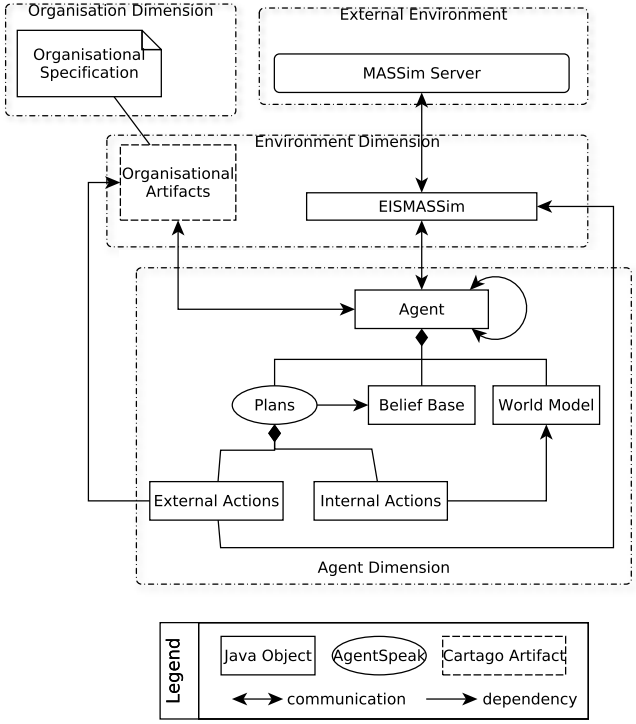
\includegraphics[width=0.7\linewidth]{./images/arquitetura.png}
\caption{Arquitetura dos times LTI-USP e ALM.}
\label{fig:arquitetura}
\end{figure}

O arcabouço CArtAgO foi utilizado para acessar os artefatos organizacionais disponíveis em Moise. CArtAgO é um arcabouço para programação de ambientes baseada em Agentes \& Artifacts (A\&A) para desenhar e modelar sistemas multi-agentes. Ele inclui várias metáforas baseadas em ambientes cooperativos de sociedades humanas, tais como: agentes como entidades computacionais que executam uma tarefa (análogo a trabalhadores humanos); artefatos como recursos; e ferramentas dinamicamente construídas para o uso e manipulação dos agentes na execução de suas tarefas. Cada artefato pode ser usado e manipulado pelos agentes em tempo de execução \cite{ricci2011cartago}. Nesse trabalho não foram desenhados novos artefatos para o uso dos agentes, tal qual o trabalho no qual o presente projeto é baseado os únicos artefatos existentes são os relacionados ao modelo organizacional feito em Moise.

Moise é um modelo organizacional para sistemas multi-agentes baseado em três dimensões: estrutural, funcional e normativa. A dimensão estrutural é construída sob três níveis. O nível individual responde pelo comportamento que um agente adota ao assumir determinado papel. O nível social diz respeito à relação entre papeis e comunicação. E o nível coletivo responde pela agregação de papéis em grupos. A dimensão funcional é formada por planos, metas e missões que representam a forma pela qual o sistema multi-agentes alcança o seu objetivo global. O objetivo global é decomposto em planos, que são distribuídos aos agentes na forma de missões, quando um agente recebe uma missão ele se responsabiliza por todas as metas que compõem a missão. E a dimensão normativa, ou deôntica, abrange a autonomia dos agentes, especificando o que é ou não permitido dentro da organização. A especificação dessa dimensão diz respeito às permissões e obrigações relacionadas a um papel. O modelo em Moise permite ao desenvolvedor delimitar as restrições da sociedade de agentes, e também pode ser usada para que os agentes raciocinem em relação a sua organização \cite{hubner2010moise}.

Os agentes se comunicam com o servidor MASSim por meio da interface EISMASSim, baseada em EIS, e distribuída pela organização da competição. Para realizar a comunicação com a interface do servidor com a competição a arquitetura padrão foi alterada pelo time LTI-USP para atuar não somente em artefatos do CArtAgO, como também no ambiente EIS.

\section{Estratégias}\label{sec:strategies}

O cenário do MAPC define cinco tipos diferentes de agentes, cada um com sua especialidade: explorador, reparador, sabotador, sentinela e inspetor. Cada classe de agente tem um conjunto de ações que lhe são permitidas, a Tabela \ref{table:tab1} exibe qual o conjunto de ações permitidas para cada tipo de agente.

\begin{table}[h]
\centering
\begin{tabular}{|c|c|c|c|c|c|}
	\hline
	         & explorador & reparador & sabotador & sentinela & inspetor \\ \hline
	\textit{recharge} &      X      &     X      &     X      &    X       & X \\ \hline
  \textit{attack}  &            &           &     X      &           &  \\ \hline
  \textit{parry}   &            &     X      &    X       &    X       &  \\ \hline
  \textit{goto}   &     X       &     X      &   X        &    X       & X  \\ \hline
  \textit{probe}   &     X       &           &           &           &  \\ \hline
  \textit{survey}  &      X      &     X      &    X       &    X       & X \\ \hline
  \textit{inspect}  &            &           &           &           &  X\\ \hline
  \textit{buy}    &     X       &     X      &     X      &   X        & X \\ \hline
  \textit{repair}  &            &      X     &           &           &  \\ \hline
  \textit{skip}   &    X        &     X      &    X       &   X        & X \\ \hline
\end{tabular}
\caption{Conjunto de ações por agente definido pelo MAPC.}
\label{table:tab1}
\end{table}

Usando como base o time LTI-USP, os papeis assumidos por nossos agentes não são diretamente mapeáveis para os times definidos para a competição. Assim tipos adicionais de agentes foram definidos de acordo com a estratégia usada. Cada papel tem uma missão associada que pode ser assumida por um ou mais tipos de agente. O time LTI-USP define alguns tipos diferentes de agentes: \textit{map\_explorer} (explorador), \textit{map\_explorer\_helper} (explorador), \textit{soldier} (todos os tipos), \textit{guardian} (sabotador), \textit{medic} (reparador), \textit{zone\_explorer} (explorador), \textit{saboteur} (sabotador), \textit{sentinel} (sentinela), \textit{repairer} (reparador), \textit{coordinator} (nenhum). Uma descrição detalhada de cada tipo pode encontra-se em \cite{franco2013improving}.

Em relação ao modelo de agentes utilizado pelo time LTI-USP, o time ALM muda um pouco a estrutura e os tipos utilizados. Nossa abordagem não utiliza os agentes do tipo \textit{guardian}, optando por uma estratégia mais agressiva de ataque possuindo mais agentes do tipo \textit{saboteur} com a missão exclusiva de eliminar oponentes. Seguindo essa linha, devido ao maior número de agentes do tipo \textit{saboteur} atacando preferimos transferir um agente do tipo \textit{soldier} responsável por manter as zonas ocupadas, para o tipo \textit{repairer} no grupo de ataque, para prestar assistência aos agentes \textit{saboteur}. A Figura \ref{fig:fig2} mostra como ficou o modelo Moise após essas alterações.
 

\begin{figure}[!ht]
\centering
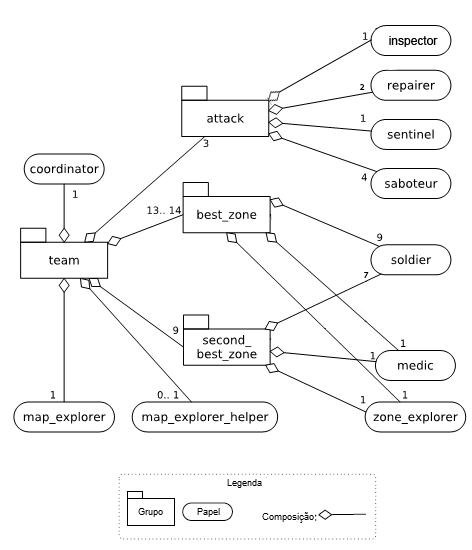
\includegraphics[width=0.7\linewidth]{./images/fig2.png}
\caption{Modelo Moise dos tipos de agente utilizados pelo time ALM}
\label{fig:fig2}
\end{figure}

\section{Experimentos}

As partidas no ambiente MAPC acontecem em mapas gerados aleatoriamente dados parâmetros que definem o número de arestas e vértices. Cada time joga três vezes um contra o outro em partidas que duram 750 passos. Para os experimentos realizados neste trabalho escolheu-se reduzir o número de passos para 200, visto que nos experimentos realizados um dos times já havia vencido até esse passo.

Os experimentos realizados colocaram o time ALM para competir contra o time LTI-USP que ficou em terceiro lugar na competição MAPC de 2013. Os times competiram em quatro ambientes diferentes definidos pelas propriedades apresentadas na Tabela \ref{table:ambientes}. Foram testados também ambientes com diferentes quantidades de vértices e arestas. A coluna semente define a semente utilizada para se gerar os mapas. Também é possível encontrar os arquivos de configuração utilizados no repositório de código deste trabalho \footnote{Repositório de Código: https://github.com/mfstabile/PCS5703}. A Figura \ref{fig:ambientes-testes} apresenta a representação gráfica dos ambientes utilizados nos testes.

\begin{table}[!h]
\centering
\begin{tabular}{|c|c|c|c|c|c|}
  \hline
             & Vértices & Arestas & N. Zonas &    Semente    \\ \hline
  Ambiente 1 &   500    &   40\%  &          & 1402107246426 \\ \hline
  Ambiente 2 &   500    &   40\%  &          & 1402129496795 \\ \hline
  Ambiente 3 &   600    &   10\%  &          & 1402141987750 \\ \hline
  Ambiente 4 &   400    &   20\%  &          & 1402235674563 \\ \hline
\end{tabular}
\caption{Conjunto de ações por agente.}
\label{table:ambientes}
\end{table}

\begin{figure}[!ht]
      \centering
      \begin{subfigure}[b]{0.48\textwidth}
              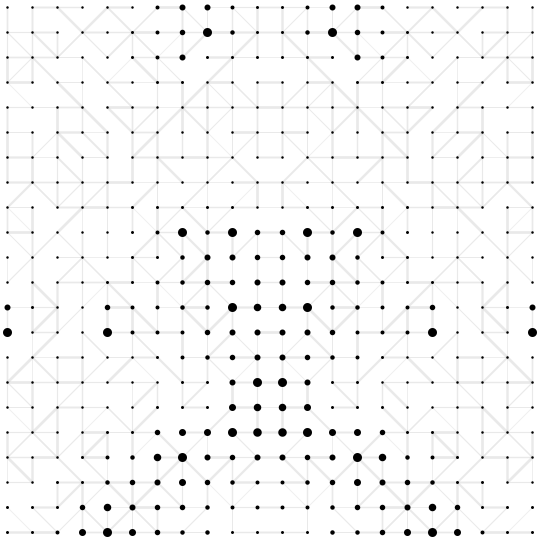
\includegraphics[width=\textwidth]{images/sim1.png}
              \caption{Ambiente 1}
              \label{fig:ambiente1}
      \end{subfigure}
      ~
      \begin{subfigure}[b]{0.48\textwidth}
              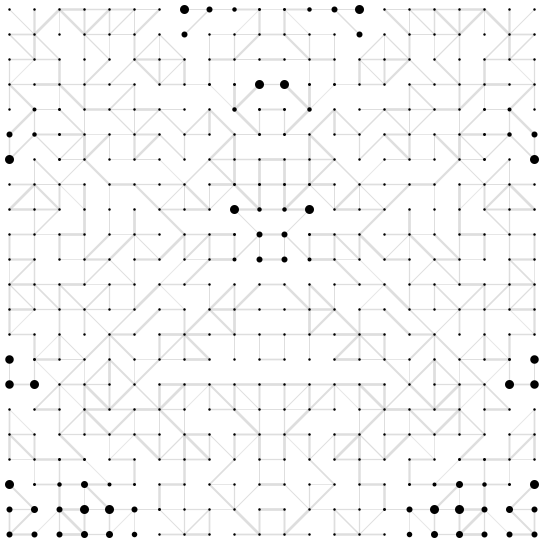
\includegraphics[width=\textwidth]{images/sim2.png}
              \caption{Ambiente 2}
              \label{fig:ambiente2}
      \end{subfigure}
      ~
      \begin{subfigure}[b]{0.48\textwidth}
              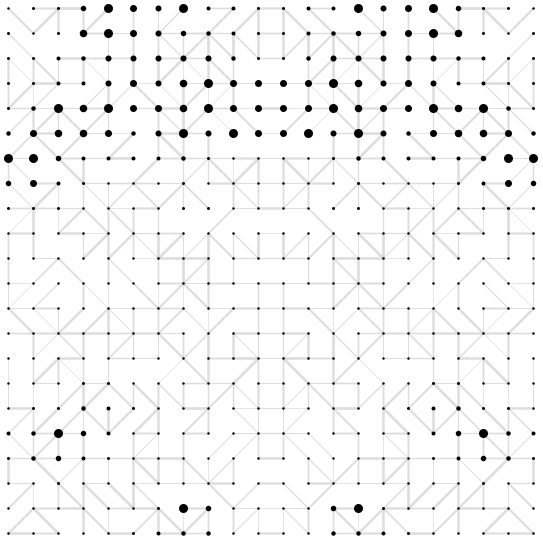
\includegraphics[width=\textwidth]{images/sim3.png}
              \caption{Ambiente 3}
              \label{fig:ambiente3}
      \end{subfigure}
      ~
      \begin{subfigure}[b]{0.48\textwidth}
              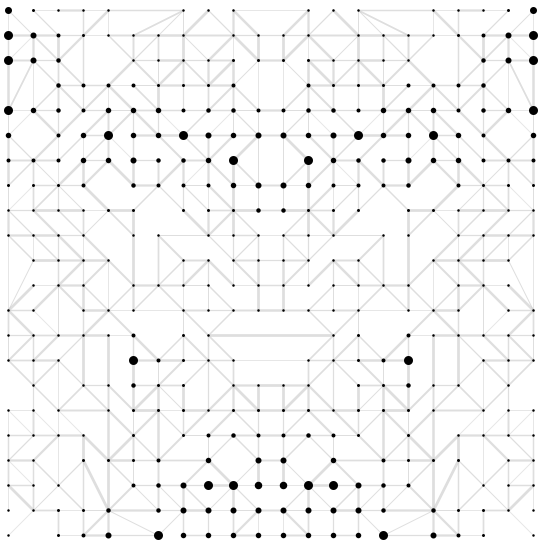
\includegraphics[width=\textwidth]{images/sim4.png}
              \caption{Ambiente 4}
              \label{fig:ambiente4}
      \end{subfigure}
      \caption{Ambientes testados nos experimentos}
      \label{fig:ambientes-testes}
\end{figure}

\section{Análise dos Resultados}

Para cada ambiente apresentado foram realizados 10 simulações de jogos entre os times ALM e LTI-USP. A Figura \ref{fig:resultados} apresenta a pontuação final dos times nos jogos para os quatro ambientes.

\begin{figure}[!ht]
\centering
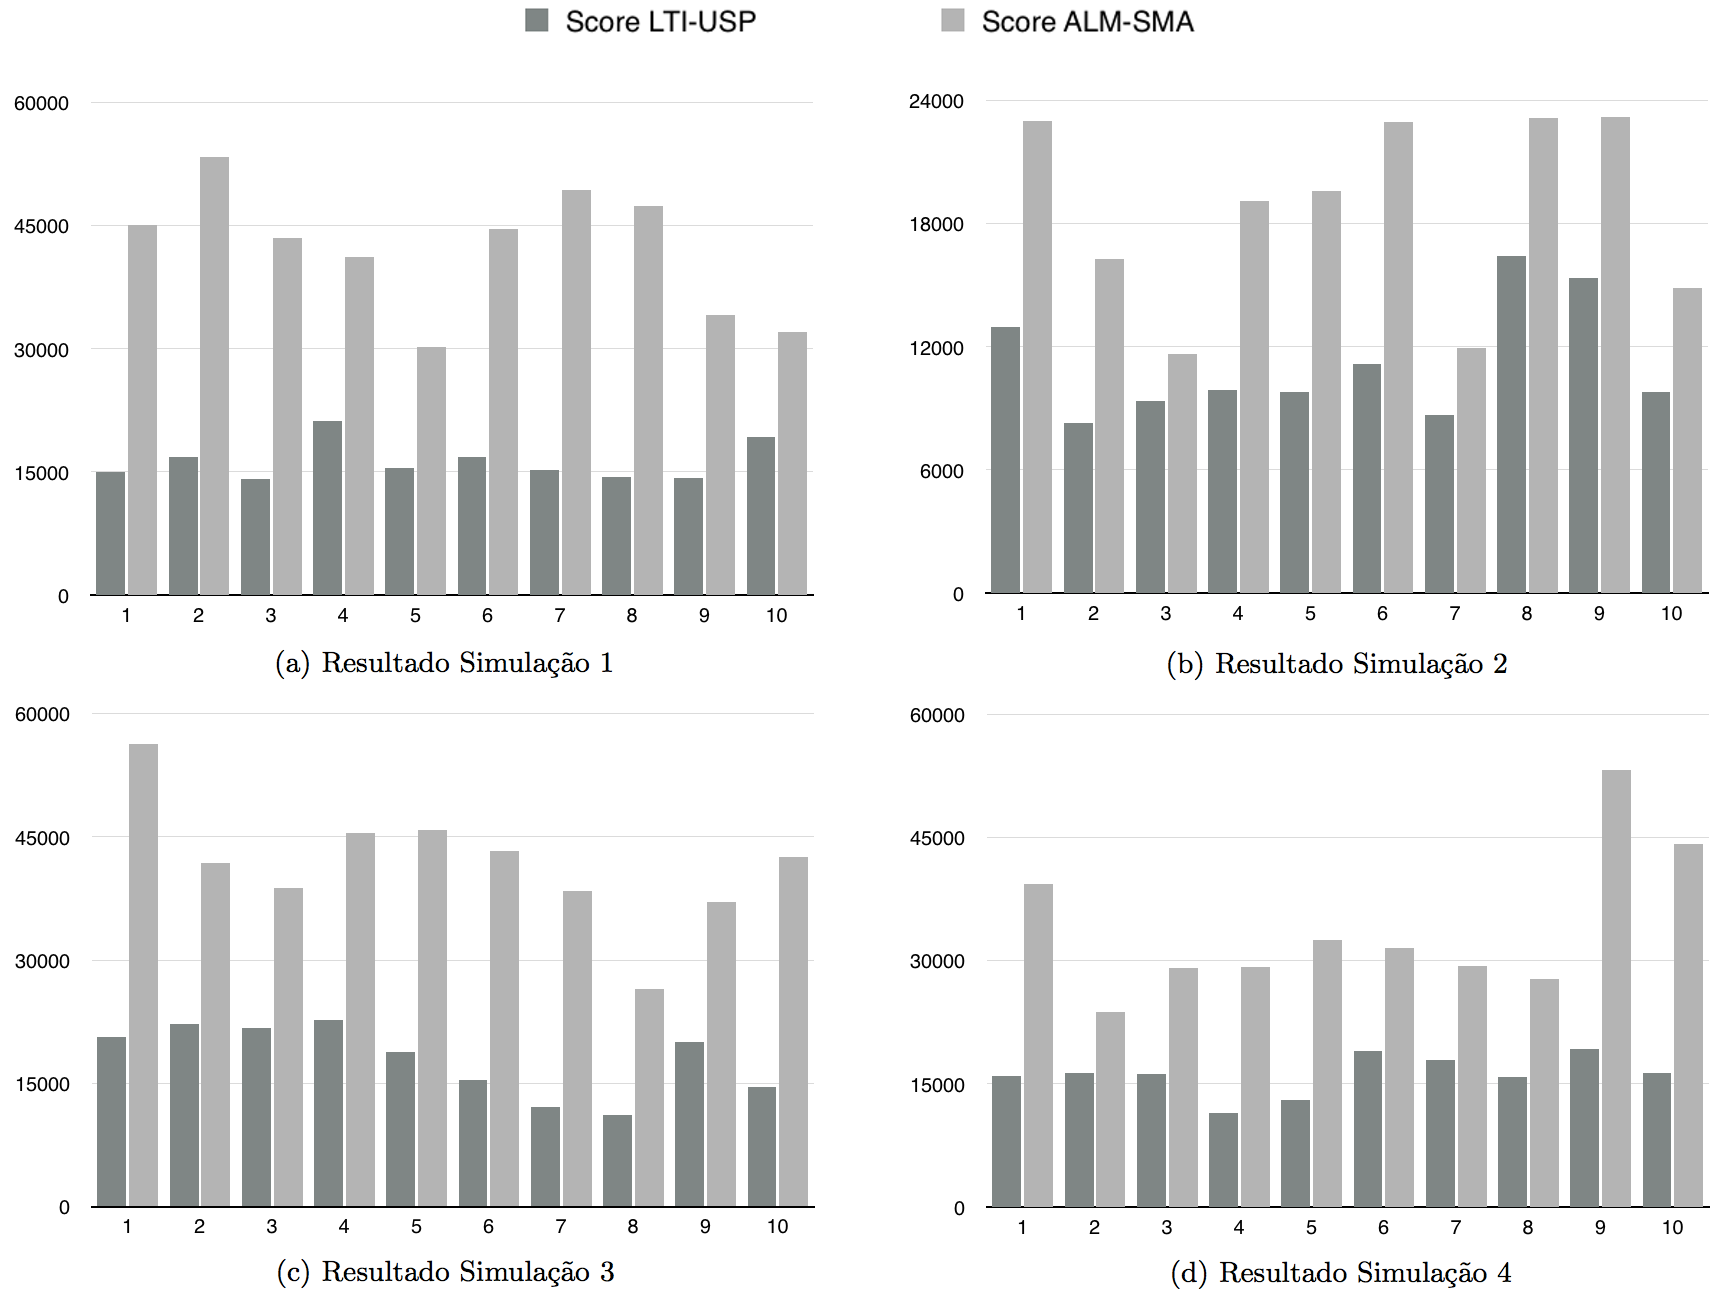
\includegraphics[width=1\linewidth]{./images/simulations-chart.png}
\caption{Resultado das simulações realizadas}
\label{fig:resultados}
\end{figure}

\textcolor{red}{WILCOXON TEST}

Como se pode notar, a alteração realizada no time ALM garantiu a vitória do time nos quatro ambientes simulados. O time ALM não possui agentes guardiões para defender as áreas conquistadas. Estes agentes foram alterados para procurar e atacar os agentes do time adversário, ficando o time com 4 agentes sabotadores com o objetivo de atacar. O time também possui dois agentes para reparar os sabotadores.

O time ALM obteve as menores pontuações no ambiente 2, seguido do ambiente 1. Podemos inferir que o fato destes ambientes possuírem zonas dispersas colaborou para a menor pontuação. O ambiente 2 possui ainda zonas muito pequenas, dificultando que os agentes consigam atingir pontuações maiores. No ambiente 2 também os agentes do time LTI-USP tiveram a disputa mais acirrada com os agentes do time ALM. Acreditamos que isto aconteceu pois a quantidade de zonas presentes no ambiente deixou os times afastados.


% \begin{figure}[ht]
%       \centering
%       \begin{subfigure}[b]{0.48\textwidth}
%               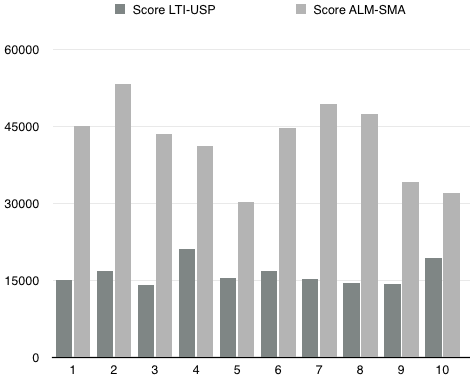
\includegraphics[width=\textwidth]{images/simulation1-chart.png}
%               \caption{Resultado Simulação 1}
%               \label{fig:resultado1}
%       \end{subfigure}
%       ~
%       \begin{subfigure}[b]{0.48\textwidth}
%               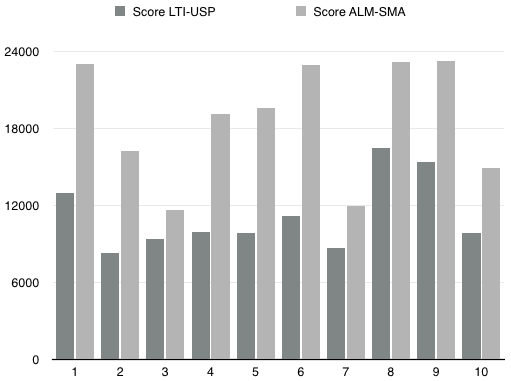
\includegraphics[width=\textwidth]{images/simulation2-chart.png}
%               \caption{Resultado Simulação 2}
%               \label{fig:resultado2}
%       \end{subfigure}
%       ~
%       \begin{subfigure}[b]{0.48\textwidth}
%               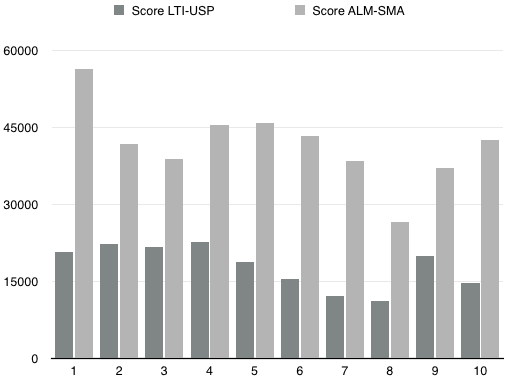
\includegraphics[width=\textwidth]{images/simulation3-chart.png}
%               \caption{Resultado Simulação 3}
%               \label{fig:resultado3}
%       \end{subfigure}
%       ~
%       \begin{subfigure}[b]{0.48\textwidth}
%               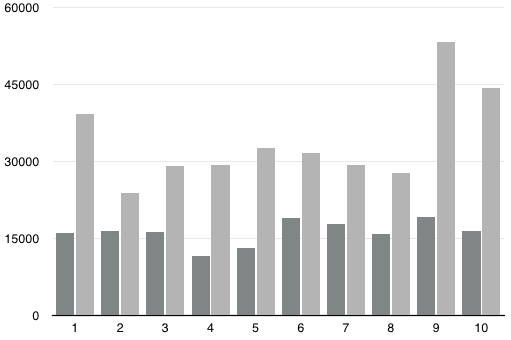
\includegraphics[width=\textwidth]{images/simulation4-chart.png}
%               \caption{Resultado Simulação 4}
%               \label{fig:resultado4}
%       \end{subfigure}
%       \caption{Resultado das simulações realizadas}
%       \label{fig:ambientes-resultados}
% \end{figure}
\section{Conclusion}
\begin{enumerate}
\item What have you learned from the participation in the contest?
\item Which are the strong and weak points of the team?
\item How suitable was the chosen programming language, methodology,
  tools, and algorithms?
\item What can be improved in the context for next year?
\item Why did your team perform as it did? Why did the other teams perform better/worse than you did.
\item Which other research fields might be interested in the Multi-Agent Programming Contest?
\item How can the current scenario be optimized? How would those optimization pay off?
\end{enumerate}

\bibliography{references}{}
\bibliographystyle{plain}

\end{document}

